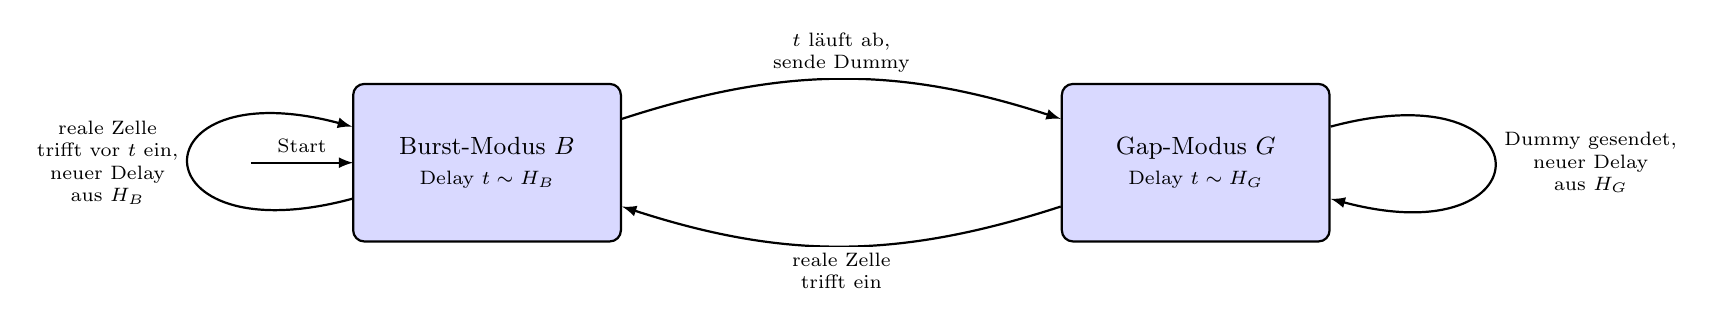
\begin{tikzpicture}[
    >=latex,
    every node/.style={font=\small},
    state/.style={
        draw, thick, rounded corners=4pt,
        minimum width=34mm, minimum height=20mm,
        align=center, fill=blue!15
    },
    edge/.style={->, thick},
    elabel/.style={
        font=\scriptsize, align=center,
        fill=white, inner sep=2pt
    },
    looplbl/.style={font=\scriptsize, align=center}
]

% Start-Pfeil in den Burst-Modus
\draw[edge] (-30mm, 0mm) -- node[font=\scriptsize, above] {Start} (-17mm, 0mm);

% Zustaende
\node[state] (B) at (0mm,  0mm)
    {Burst-Modus $B$\\\scriptsize Delay $t \sim H_B$};
\node[state] (G) at (90mm, 0mm)
    {Gap-Modus $G$\\\scriptsize Delay $t \sim H_G$};

% Transition B -> G (oben)
\draw[edge] (B) to[bend left=18]
    node[elabel, above] {$t$ läuft ab,\\sende Dummy} (G);

% Transition G -> B (unten)
\draw[edge] (G) to[bend left=18]
    node[elabel, below] {reale Zelle\\trifft ein} (B);

% Selbst-Schleife B (links)
\draw[edge] (B) edge[loop left, looseness=8]
    node[looplbl, left, align=center]
    {reale Zelle\\trifft vor $t$ ein,\\neuer Delay\\aus $H_B$} (B);

% Selbst-Schleife G (rechts)
\draw[edge] (G) edge[loop right, looseness=8]
    node[looplbl, right, align=center]
    {Dummy gesendet,\\neuer Delay\\aus $H_G$} (G);

\end{tikzpicture}
